\documentclass{hotnets16}

% Comment out the following line to disable comments
\def\commentenabled{1}

\usepackage{times}  
\usepackage{epsfig}
\usepackage[TABBOTCAP]{subfigure}
\usepackage{tabularx}
\usepackage{graphicx} 
\usepackage{color}
\usepackage{xspace}
\usepackage{thumbpdf}
\usepackage{listings}
\usepackage{verbatim}
\usepackage{hyperref}
\usepackage{booktabs}
\usepackage{colortbl}
\usepackage{caption}
\usepackage{todonotes}
\usepackage{mathtools}
\usepackage{amsmath}
\usepackage{cleveref}
\usepackage{eqnarray}

\newtheorem{property}{Property}
\newtheorem{theorem}{Theorem}

\newcommand{\minisection}[1]{\smallskip\noindent{\bf #1.}}
\newcommand{\secref}[1]{{\S\ref{#1}}}
\newcommand{\secsref}[2]{{Sections~\ref{#1} and \S\ref{#2}}}
\newcommand{\figref}[1]{{Figure~\ref{#1}}}
\newcommand{\figsref}[2]{{Figure~\ref{#1} and \ref{#2}}}
\newcommand{\appref}[1]{{Appendix~\ref{#1}}}
\newcommand{\thmref}[1]{{Theorem~\ref{#1}}}
\newcommand{\lemref}[1]{{Lemma~\ref{#1}}}
\newcommand{\corref}[1]{{Corollary~\ref{#1}}}
\newcommand{\proref}[1]{{Property~\ref{#1}}}
\newcommand{\tabref}[1]{{Table~\ref{#1}}}


\newcommand{\compactcaption}[1]{\vspace{-1em}\caption{#1}\vspace{-1em}}
\newcommand{\botcompactcaption}[1]{\caption{#1}\vspace{-1em}}
\newcommand{\topcompactcaption}[1]{\vspace{-1em}\caption{#1}\vspace{-0.5em}}

\newenvironment{compactitemize}
{
   \begin{itemize}[leftmargin=1.5em]
   \vspace{-1ex}
   \setlength{\topsep}{0pt}
   \setlength{\itemsep}{0em}
   \setlength{\parskip}{0pt}
   \setlength{\parsep}{0pt}
}
{
   \vspace{-1ex}
   \end{itemize}
}
\newenvironment{compact2itemize}
{
	\begin{itemize}[leftmargin=1.5em]
		\vspace{-1ex}
		\setlength{\topsep}{0pt}
		\setlength{\itemsep}{0.5em}
		\setlength{\parskip}{0pt}
		\setlength{\parsep}{0pt}
	}
	{
		\vspace{-1ex}
	\end{itemize}
}


\newenvironment{compactenumerate}
{
   \begin{enumerate}[leftmargin=1.5em]
   \vspace{-1ex}
   \setlength{\topsep}{0pt}
   \setlength{\itemsep}{0em}
   \setlength{\parskip}{0pt}
   \setlength{\parsep}{0pt}
}
{
   \vspace{-1ex}
   \end{enumerate}
}


\hypersetup{pdfstartview=FitH,pdfpagelayout=SinglePage}

\setlength\paperheight {11in}
\setlength\paperwidth {8.5in}
\setlength{\textwidth}{7in}
\setlength{\textheight}{9.25in}
\setlength{\oddsidemargin}{-.25in}
\setlength{\evensidemargin}{-.25in}
%\setlength{\headsep}{0in}
%\pagenumbering{arabic}

\begin{document}

\conferenceinfo{HotNets 2016} {}
\CopyrightYear{2016}
\crdata{X}
\date{}

%%%%%%%%%%%% THIS IS WHERE WE PUT IN THE TITLE AND AUTHORS %%%%%%%%%%%%

\title{Policy Enforcement using \\ Distributed Control Plane Synthesis}

\author{Anonymous}

\maketitle

%\thispagestyle{empty}

%%%%%%%%%%%%%  ABSTRACT GOES HERE %%%%%%%%%%%%%%
\subsection*{Abstract}

Synthesizing ARCs ...

\section{Introduction}

Network operators of enterprise and cloud datacenter networks deal
with thousands of flow groups traversing large number of heterogeneous
devices. With growing diversity of applications, need for security and
compliance, and the advent of cloud comouting, these flow groups may
be subject to increasingly complex policies. Cloud tenants or
enterprises require basic reachability between hosts/application, and
middlebox traversal for certain flow groups. Operators, on top of that
require support for policies like traffic isolation between flows to
provide security and fairness, and satisfying resource constraints
pertaining link bandwidths and switch table sizes to perform traffic
engineering and network resource management.  However, configuring
network devices to implement these diverse and complex policies is
manual, ad-hoc and error prone today, leading to violations of
service-level agreements and mis-configurations which have severe
performance and security impacts.

%%  However, in real-life, the
%% process of policy enforcement by network operators is manual and
%% ad-hoc, leading to violations of service-level agreements and
%% mis-configurations which have severe performance and security
%% impacts. With the boom in cloud services, datacenter networks deal
%% with thousands of flows which are not constant, but in flux, thus,
%% making it difficult to enforce them in an ad-hoc manner.

%% Network operators desire various different end-to-end policies to
%% support in clouds and enterprise networks. Tenants or organisations
%% require support for basic policies like reachability between hosts,
%% and specifying different middlebox policies for certain
%% flows. Operators, on top of that require support for complex policies
%% like traffic isolation between flows to provide fairness and
%% specifying resource constraints like link bandwidth and switch table
%% sizes to perform traffic engineering and network resource management.

Though Software-defined Networking (SDN) has allowed network operators
to program networks in a more intuitive manner, many of existing SDN
tools/frameworks are too low-level in their functionality. Supporting
the aforementioned types of policies simply using SDN-capable switches
or with existing languages like Frenetic~\cite{frenetic} and
Pyretic~\cite{pyretic} is extremely challenging; operators would
ideally want to specify and realize policies network-wide without
programming individual switch behaviors. \aditya{we need to be careful
  not to bin all SDN languages into this switch-by-switch model}.
There has been research in the field of network-wide policy
enforcement in networks, like bandwidth provisioning in Merlin
\cite{Merlin}, and middlebox policy enforcement in SIMPLE
\cite{simple} or FlowTags~\cite{flowtags}. However, these approaches
are tailor-made to specific policies, and thus, difficult to extend it
to support other kinds of policies.

In this paper, we seek a {\em general} approach, where operators can
specify a variety of custom policies in a simple, declarative way, and
the complexities of correctly realizing the policies in the data plane
are hidden away from them. %% To support a cornucopia of policies, an
%% important feature is \emph{generality} of the approach of policy
%% enforcement, so that it can be extended to enforce custom policies
%% required by the operator.
By designing and implementing a system called \Name, this paper makes
a case for using \emph{efficient synthesis} of switch table forward
rules to realize this vision.
%% switch
%% table forwarding rules to the solve the problem of policy enforcement
%% by use of off-the-shelf SMT-solvers.

We show that enforcement of several of the policies supported by
\Name, specifically isolation, and middlebox traversal is
NP-complete. Thus, \Name leverages recent advances in creating fast
SMT solvers (e.g., Z3~\cite{z3}) to perform synthesis by encoding the
policy enforcement problem to a SMT instance, and using the SMT solver
to search for a solution, which is then translated into switch
rules. %% This paper presents Genesis, a
%% network management tool where the network operators can express the
%% network-wide policies in a high-level declarative manner and Genesis
%% will synthesize the lower-level switch forwarding rules for realising
%% these policies, eliminating the need for operators to work on
%% switch-level behaviours.
By leveraging a formal reasoning technique of SAT/SMT solving, \Name
eliminates the room for error in policy enforcement.

Unfortunately, naive application of SMT solvers results in synthesis
speeds that don't match the scale of operations of cloud and
enterprise networks today. \aditya{give an example as to how slow
  things can get} To overcome this challenge, \Name leverages a few
domain-specific ideas.  Specifically, it uses a novel search strategy
using regular expressions to prune the space of forwarding plane
configurations by leveraging data center network
structure. \aditya{the previous sentence is vague} knowlegde. Second,
\Name uses heuristical synthesis routine that leverages the nature of
policy interactions to improve synthesis performance. \aditya{quickly
  talk about in 1-2 sentences the speedup achieved with these
  optimizations}

%% are
%% huge, and by supporting a set of diverse and complex policies with
%% different search objectives, we require to create a model general and
%% expressive enough to support these. This poses a challenge as to can
%% synthesis performance be improved by leveraging knowledge specific to
%% the problem of policy enforcement in networks?

We implement \Name using ... We evaluate it using .... Key highlights .... \aditya{all of these are todo}.

Thus, the main contribution of this paper are: \aditya{todo}

%% : We present the design and implementation of a network management
%% system with support for a diverse set of complex end-to-end
%% policies like isolation, waypoints and capacity. We designed a
%% novel search strategy using regular expressions to prune the space
%% of forwarding plane configurations by leveraging the network
%% structure to provide properties of the path, especially in
%% datacenter topologies. Lastly, we design a heuristical synthesis
%% routine leveraging the nature of policy interactions to improve
%% synthesis performance.

\input{Motivation}

% \section{Related Work}
% --- Fill In Later ---
% % Fibbing: Lies can cause loops if the centralized controller fails,
% % our approach is sounder

% <Write about ARC here because people may not have read about it yet>

\section{Control Plane Synthesis via ARCs} \label{sec:synthesis}
In this section, we describe preliminary ideas on how each phase of our synthesis 
approach can be implemented.
First, we briefly discuss how existing tools can be used to generate
policy-compliant paths (\secref{phase1}).
Second, we show how to generate ARCs that induce
the set of paths synthesized in the first phase (\secref{phase2}).
Third, we show how ARCs can be modified to deal with resilience (\secref{TODO}).
Finally, we show how to restart the process whenever one of the three phases fails (\secref{TODO}).

\subsection{From policies to paths} \label{sec:phase1}
The first phase of our approach produces a set of paths adhering to
different policies like reachability, service chaining, traffic engineering and isolation.
Synthesizing sets of paths---i.e., data planes---that adhere to a given set of policies
is already a hard problem, but a few practical approaches have been proposed.
The approach that is most similar to ours is the one used in Merlin~\cite{merlin}.
Given a set of waypoints, reachability, and bandwidth guarantee policies,
Merlin generates a mixed integer linear programming instance. 
A solution to this instance is a set of paths meeting the input policies.
Our prototype implementation uses a similar idea and,
since this part of the problem is not novel, we briefly provide the intuition behind our solution.
Given a set of policies we generate a set of constraints over the propositional theory of rationals 
and the solutions to these constraints are paths satisfying all the policies.
Our rich policy language requires complex Boolean reasoning that forces us to adopt propositional theories
in place of simple conjunctions of constraints.
In particular, policies like isolation and waypoints require disjunctive formulas.

%\loris{we will add more details if needed}


\subsection{From paths to ARCs} \label{sec:phase2}

The second phase of our approach takes as input the set of paths produced by the first phase
and produces an Abstract Representation of the Control Plane (ARC) that realizes the given set of paths.
First, we consider the problem of generating ARCs that
 forward packets based on shortest-paths---e.g., OSPF routing.
Then, we consider more complex forms of ARCs in which 
 additional mechanisms like route-filtering are allowed. 
 
\subsubsection{From paths to simplified ARCs}
The \emph{Simplified Abstract Representation of the Control Plane} (sARC) is a directed graph comprising switches as 
vertices and weighted edges corresponding to all links in the
topology. 
This is an ideal control plane supporting classic shortest path routing in which no links can be disabled. 

The problem of synthesizing 
a sARC that realizes an input set of paths reduces to a
variation of the so-called {\em inverse shortest path} problem~\cite{isp}. 
Assume we are given the following inputs: (1) a directed graph $T = (S, L)$ (the network topology), 
(2) a set of endpoints $\Gamma \subseteq S\times S$
describing the sources and destinations of the input paths, and 
(3) a function $P: \Gamma \rightarrow 2^{L^*}$
that assigns to each pair of endpoints $(s,t) \in \Gamma$ 
a set of \emph{acyclic} paths, such that for every path $l_0\cdots l_n\in P(s,t)$,
$l_0=(s,s')$, for some $s'\in S$, and $l_n=(s'',t)$, for some $s''\in S$.\footnote{
We use $L^*$ the denote the set of all finite sequences over the set $L$.}
The 
\emph{sARC synthesis}
problem is to find rational weights for the edges in $L$ such that 
for each pair of endpoints $(s,t) \in \Gamma$, 
the paths in $P(s,t)$ are \emph{the} shortest paths from $s$ to $t$ 
in the graph. Notice, that there can be multiple shortest
paths of equal cost for multi-path support (e.g., for traffic engineering).

In sARC, packet forwarding is based on destination.
For a destination $d$, we call $\xi_d$ the directed
subgraph of $T$ obtained by only keeping the nodes and edges 
that are traversed by paths with destination $d$.
Since paths are acyclic, $\xi_d$ is a directed acyclic graph.
We use $\Omega=\{d\mid (\_,d)\in\Gamma\}$ to denote the 
set of all destinations and $\Delta=\{\xi_d\mid d\in \Omega\}$ to denote  
the set of all destination DAGs. 

We use  $sw_1\rightarrow sw_2$ to denote $(sw_1,sw_2)\in L$ and
$sw_1\rightarrow^* sw_2$ (resp. $sw_1\rightarrow^+ sw_2$) to denote 
that $sw_2$ is reachable from $sw_1$ by crossing zero (resp. one) or more links in $T$.
Similarly, we use $\rightarrow_{\xi_d}$ to denote the same relations in the destination DAGs.


\minisection{Distance Equations}
To solve the sARC synthesis problem, we generate a set of linear equations
to find the required edge weights. 
We use $E(sw_1, sw_2)$ to denote the weight of the edge $(sw_1,sw_2)\in L$
and 
$D(sw_1, sw_2)$ to denote the shortest distance from $sw_1$ to $sw_2$.
We add the equation $D(s,s) = 0$ for every $s\in S$ to denote that the distance
from a node to itself is $0$.
The
following equation guarantees that $D(s,t)$ is not greater than 
the actual shortest distance from $s$ to $t$.
\begin{multline} \label{eq:dist}
\forall s, t, sw. (s \rightarrow sw \rightarrow^* t).\\
D(s, t) \leq E(s, sw) + D(sw, t)
\end{multline}

For each destination DAG $\xi_d\in\Delta$, we add equations to ensure 
that the input paths with destination $d$ are indeed the shortest ones.
 If a path
is the shortest path between its endpoints, then every 
subpath of the path has to be the shortest between its endpoints
as well (otherwise the complete path would not be the shortest).
\begin{figure}[h!] 
	\centering
	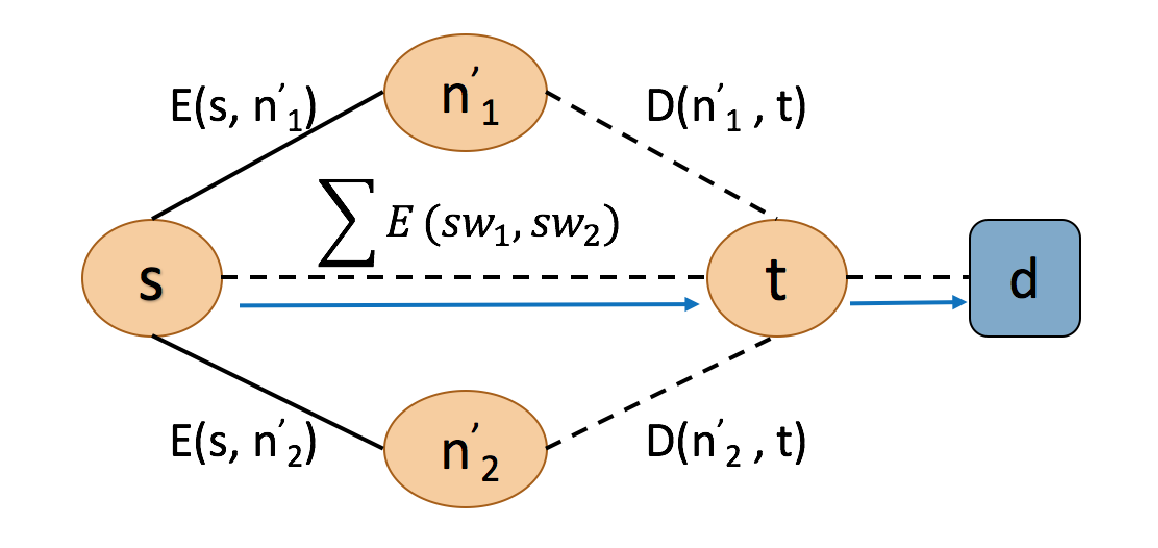
\includegraphics[width=0.8\columnwidth]{figures/distanceEquation.eps}
	\caption{An example illustration of the distance equations for shortest path forwarding.
		The pointed arrows represent the path in DAG of destination $d$, and the
		dotted line represents 1 or more edges. 
	} \label{fig:disteq}
\end{figure}
Consider a DAG $\xi_d$ for destination $d$. We define two neighbour
functions: $N_T(s)$ denotes the set of neighbours of switch $s$ 
in the input graph $T$, and $N_{\xi_d}(s)$ denote the set of
neighbours of switch $s$ in the destination DAG $\xi_d$. 
Given a destination $d\in \Omega$,
we use the following equations to ensure that, given two nodes $s$ and $t$ in
$\xi_d$, 
the set of paths from $s$ to $t$ in $\xi_d$ are
exactly
\emph{the} shortest paths from $s$ to $t$ in $T$ (\Cref{fig:disteq} illustrates 
an example).
Let $s,t$ be two nodes in $\xi_d$ and let  $Paths_{\xi_d}(s,t)$ be the set of paths from $s$ to $t$ in $\xi_d$.
\begin{multline} \label{eq:uniq1}
		\forall l_0\cdots l_n\in Paths_{\xi_d}(s,t).
		\forall n' \in N(s) \setminus N_{\xi_d}(s). \\
		E(s, n') + D(n', t) > \sum_{\mathclap{\substack{l_i=(s_i,t_i)}}} 
		E(s_i, t_i) 
\end{multline}
\begin{multline} \label{eq:uniq2}
		\forall l_0\cdots l_n\in Paths_{\xi_d}(s,t).
		\forall n' \in N_{\xi_d}(s). n' \not\rightarrow^+_{\xi_d} t.  \\
		E(s, n') + D(n', t) > \sum_{\mathclap{\substack{l_i=(s_i,t_i)}}} 
		E(s_i, t_i) 
\end{multline}
\begin{multline} \label{eq:uniq3}
		\forall l_0\cdots l_n, l_0'\cdots l_n'\in Paths_{\xi_d}(s,t).\\
		\sum_{\mathclap{\substack{l_i=(s_i,t_i)}}} 
		E(s_i, t_i)  =\sum_{\mathclap{\substack{l_i'=(s_i',t_i')}}} 
		E(s_i', t_i') 
\end{multline}
Equation~\ref{eq:uniq1} guarantees that 
the sum of the weights belonging to a path from $s$ to $t$ in $\xi_d$ is smaller than 
any path that goes to $t$ via a node $n'$ that is a neighbour of $s$ in $T$ but not in $\xi_d$.
Equation~\ref{eq:uniq2} guarantees that
the sum of the weights belonging to a path from $s$ to $t$ in $\xi_d$ is smaller than 
any path that goes to $t$ via a node $n'$ that is a neighbour of $s$ in $\xi_d$ but such that
$t$ is not reachable from $n'$ in $\xi_d$.
Finally, Equation~\ref{eq:uniq2} guarantees that all the paths from $s$ to $t$ in $\xi_d$ have the same weight.

% If the path $n' \rightarrow^* t$ 
% is not in any DAG completely, then
% $D(n',t)$ can be smaller than the actual shortest distance by the
% semantics of \Cref{eq:dist} (as
% $D(n',t)$ is not equal to any quantity by \Cref{eq:shortest}).
% However, since $D(n',t)$ is on the RHS of the equations in \Cref{eq:uniq},
% the equations will ensure that the path $s\rightarrow n \rightarrow^* t$
% has strictly greater weight than the path of the DAG.

%TODO: Add some figures

\subsubsection{Synthesis of ARC with route-filters} \label{sec:routefilter}
\begin{figure}
	\centering
	\begin{tikzpicture}[shorten >=0.5pt,node distance=,on grid,auto,
	square/.style={regular polygon,regular polygon sides=4}] 
	\node[state] at (0,0) (s)  {$s$}; 
	\node[state] at (2,0.5) (v1)  {$r_1$}; 
	\node[state] at (2,-0.5) (u1) {$r_2$}; 
	\node[state] at (4, 0)(t) {$t$};
	\node[state, rectangle] at (6, -0.75) (d2) {$\lambda_2$};
	\node[state, rectangle] at (6, 0.75) (d1) {$\lambda_1$};
	\path[->] 
	(s) edge  node {} (v1)
	edge  node {} (u1)
	edge [blue, dashed, bend right=45] node {} (t)
	edge [red, dashed, bend left=45] node {} (t)
	(u1) edge node {} (t)
	(v1) edge node {} (t)
	(t) edge [red, dashed] node {} (d1) 
	edge [blue, dashed] node {} (d2);
	\end{tikzpicture}
	\caption{Example of paths which require route-filtering. This is a
		diamond starting at $s$ and ending at $t$. The diamond can be
		eliminated by filters $((s,r_1),\lambda_2)$ or $((s,r_2),\lambda_1)$.}
	\label{fig:diamond}
\end{figure}

The sARC synthesis problem does not always admit a solution.
This blocking mechanism supported by (non-simplified)
ARC is called a route-filter. 
A route-filter  can selectively disable an
edge for a given destination by  blocking advertisements to a
particular destination along a link. 
Formally, a route-filter is a pair $(l,d)\in L\times S$
disabling a link $l$ for destination $d$
and path to a destination $d$ is \emph{unfiltered} 
if it does not contain edges that are filtered for destination $d$.
%Therefore, if a route-filter is added on switch $s3$, 
%$s3$ 
%will not advertise a route for $d1$ to $s1$, so 
%$s1$ will forward to $s2$ and not to $s3$
%to reach $d1$. The forwarding of packets destined
%for $d2$ are not affected, and they will be sent from
%$s1$ to $s4$ via $s3$ as it is the shortest path.
%Thus, by incorporating route-filters, we can
%disable certain links in the topology 
%for specific destinations, and synthesize
%ARCs for all possible data planes. 
The \emph{ARC synthesis} problem
is to find rational weights for the edges in $L$
and a set of route-filters $F\subseteq L\times S$
 such that 
for each pair of endpoints $(s,t) \in \Gamma$, 
the paths in $P(s,t)$ are the shortest \emph{unfiltered} paths from $s$ to $t$ 
in the graph. 

The ARC synthesis problem admits a trivial solution in which 
route-filters are used to enforce the exact set of input paths by blocking all other possible paths.
This can be done by creating a 
route-filter $(l,d)$ for every link $l$ not in $\xi_d$. 
However, this solution may overly restrict the structure of the network.
In particular, if two nodes were connected by a single path,
a link failure would immediately result in the network becoming disconnected!
Moreover, installing so many route-filters might be costly as not all switches might
support this mechanism.

Ideally, we would like to impose further restrictions to the ARC
synthesis problem to make sure that the obtained solution
satisfy desirable connectivity or resilience properties.
In the following we informally use the word objective 
to identify a property we desire for the synthesized ARC.
Examples of objectives are minimizing the number of route-filters
or maximizing the number of edge-disjoint paths in the ARC
for each endpoint. 
Given an objective $O$, the \emph{augmented ARC synthesis} problem
is to find rational weights for the edges in $L$
and a set of route-filters $F\subseteq L\times S$
 such that 
1) for each pair of endpoints $(s,t) \in \Gamma$, 
the paths in $P(s,t)$ are the shortest \emph{unfiltered} paths from $s$ to $t$ 
in the graph,
2) the resulting ARC satisfies the objective $O$. 
In the following we only allow route-filters for a destination $d$ to be applied to edges of $T$ that are directly connected to 
nodes in $\xi_d$. 

We propose an iterative approach to this problem. 
Our algorithm starts by trying to synthesize a solution
that does not use route-filters using the equations proposed in \secref{sec:sarc}. 
In the case of a failure, the algorithm uses the ``proof of unsatisfiability'' generated by the constraint solver 
to greedily add a small set of route-filters. New equations are then generated and approach is repeated until a solution is found.
We first describe the 
modified linear equations generated when a set of
route-filters are enabled, and then describe two
techniques used to choose route-filters. 
%\begin{figure}
%	\centering
%	\includegraphics[width=\columnwidth]{figures/arcSynthesis.eps}
%	\caption{Synthesis of ARC with route-filters.} \label{fig:arcSynthesis}
%\end{figure}

\minisection{Equations with route-filters}
We show how the technique used to solve the simplified synthesis
problem can be modified to handle filtered and unfiltered paths.
We assume we are given a set of route-filters $F$ and 
use $s\rightarrow_d^* t$ to denote that $s$ can reach $t$
in $T$ without using any edge $l$, such that $(l,d)\in F$.
We use $D_d(r_1, r_2)$ to denote the shortest distance from $r_1$ to $r_2$
using only edges that are not filtered for destination $d$.
We can revise the equation in \eqref{eq:dist} to correctly restrict the values of $D_d$
by simply ignoring all the filtered edges. 
In the same way, we can modify equations  \eqref{eq:uniq1} and \eqref{eq:uniq2}, while
equation \eqref{eq:uniq3} remains unchanged.

Unfortunately, if the encoding without route-filters produces $n$ equations, this encoding produces $|\Omega|n$ due
to the multiple different distances $D_d$.
Notice that, the shortest distance $D_d(s,t)$ between two nodes $s$ and $t$ without using edges filtered for $d$ cannot be
smaller than the shortest distance $D(s,t)$ obtained without considering route-filters.
We use this property to simplify the encoding by only computing $D(s,t)$ and by replacing each instance of $D_d(s,t)$
with $D(s,t)$ in
equations \eqref{eq:uniq1} and \eqref{eq:uniq2}. 
It is easy to see that every solution of this simplified set of constraints
is also a solution to the original solution (because $D(s,t)\leq D_d(s,t)$).
However, the reverse is not true and the set of simplified equations can be unsatisfiable
in cases in which the original set is satisfiable.
We use the simplified
set of equations in our preliminary implementation and show how it yields encouraging results in practice.

If the set of linear equations does not admit a solution, we 
can add new route-filters so that the equations resulting from the added
route-filters admit a solution.
We discuss two schemes used to add route-filters:
the first scheme uses unsatisfiable cores generated
by the solver and the second scheme 
finds geometrical structures called diamonds that 
cannot be handled without route-filters.


% While detecting diamonds is efficient, the
% presence of diamonds is a not 
% necessary condition for route-filtering.
% Characterising the properties of data planes for which there is
% a pure ARC solution (i.e., no route-filters
% required) is a open algorithmic
% problem. An 
% efficient algorithm to find the structures causing 
% inconsistencies based on these properties 
% can be used to minimize the number of route-filters enabled.  

\todo{Not good, improve} \\
\minisection{Adding filters using unsatisfiable cores}
Modern LP-solvers have efficient procedures to return an
unsatisfiable core, also called IIS (Irreducible Inconsistent Subsystem)
~\cite{chinneck2007feasibility}. Formally, an IIS is a subset of constraints such that,
if all constraints except those in the IIS are removed, the resulting set of
linear equations is still inconsistent (unsatisfiable). Moreover, the set is irreducible---i.e., removing 
any one constraint of the IIS produces a consistent set of constraints. 

Suppose that, upon producing our set of linear equations, the solver returns unsatisfiable and produces
a concrete unsatisfiable core. 
Some of the linear inequalities from 
Equations \eqref{eq:uniq1} and  \eqref{eq:uniq2}
will appear in the unsat-core 
(an unsat-core cannot consist of only 
constraints from \Cref{eq:dist} and \eqref{eq:uniq3}, as all distances and edges set to zero
would trivially be consistent with these constraints). 
In particular, the unsat-core contains some constraint
\begin{eqnarray}
E(s, n') + D(n', t) > \sum_{\mathclap{\substack{l_i=(s_i,t_i)}}} 
		E(s_i, t_i) 
\end{eqnarray}
that was added to reason about some DAG $\xi_d$.

By adding the route-filter $((s,n'),d)$ to $F$, this inequality is removed from the set of constraints
and the combination of the other constraints appearing in the other unsat-core is now satisfiable.
The complete set of equations may still be inconsistent as other unsat-cores might exist. 
The procedure can be repeated until the resulting set of constraints becomes satisfiable
and we have therefore reached a solution to the ARC synthesis problem.

Finding the optimal number of route-filters is NP-hard, and it
is very difficult to incorporate optimality in our iterative learning
technique for finding the set of filters. This is because we do not 
have the set of all unsatisfiable cores (the solver returns one at 
a time) to find an optimal set of filters. Instead of considering the 
number of filters, we consider the metric: loss of resilience.
%\loris{not sure the next paragraph is needed}
%For a given unsat-core, there may be multiple ways to place a route
%filter to eliminate one constraint and we have not investigated
%We can 
%adopt a greedy approach (based on set cover \cite{setcover}) 
%of picking a route-filter which 
%eliminates the maximum number of unsat-cores. However, 
%finding the number of unsat-cores a route-filter eliminates
%is an open problem and instrumental in minimizing the number 
%of route-filters. Other schemes can be used to choose 
%a route-filter from an unsat-core satisfying certain
%objectives. 

Finding an IIS is an NP-hard problem~\cite{iiscomplexity}
and can result in slow synthesis times.
%We identify a topological property of the set of input paths that 
%is guaranteed to require route-filters and use it to produce an initial set of necessary route-filters.
%This technique allows us to reduce the number of times we are required to compute  unsat-cores.
%
%We define the structure shown in \Cref{fig:diamond}
%as a \emph{diamond}. 
%Formally, a problem instance contains a diamond iff there exists two different destinations $d$ and $d'$
%such that, in their corresponding DAGs $\xi_d$ and $\xi_{d'}$,
%there exists two nodes $s$ and $t$, such that $s\rightarrow_{\xi_d} t$,
%$s\rightarrow_{\xi_{d'}} t$, and
%there exists a path $l_0\cdots l_n$ from $s$ to $t$ in $\xi_d$ that is not a path from
%$s$ to $t$ in $\xi_{d'}$.
%As we mentioned at the beginning, synthesizing an ARC for  diamond structures requires
%the addition of a route-filter.
%In fact, each such a diamond can be ``removed'' by introducing a route-filter $(l_0, d')$ that hides
%the path $l_0\cdots l_n$ for the destination $d'$ (see \Cref{fig:diamond}).
%Diamonds can detected and removed in polynomial time.
%%Consider
%the diamond in \Cref{fig:diamond}. There are two choices
%of route-filters: the $s1-s3$ edge for destination $d1$ 
%and the $s1-s2$ edge for destination $d2$, out of which,
%at least one filter is required to eliminate the 
%inconsistency in the linear equations caused due to the diamond.
%Thus, we find all diamonds for all pairs of destination
%DAGs (this is done in polynomial time) and assign a filter
%to one of the two edges at the source of each diamond. 
%Thus, by removing the diamonds, we can reduce the 
%number of iterations
%of the unsat-core learning approach, which would have 
%provided diamonds as an unsat-core if 
%diamonds were not eliminated.





\subsection{From ARCs to resilient ARCs} \label{sec:phase3}


The \ARC synthesized using the aforementioned approach represents a control
plane that will compute policy-compliant paths in the absence of failures.
However, it does not guarantee policy compliance when failures occur. For
example, if a link along the shortest path fails, the next shortest path (if
one exists) will become the new path to reach the destination. However, the
new path may not conform to the same policies as the path in the original
failure-free data plane from which the \ARC was synthesized---e.g., the new
path may no longer traverse a waypoint or have the same bandwidth capacity.
Given the high frequency of failures in data center~\cite{datacenterfailures},
campus, and wide-area~\cite{turner10:sigcomm} networks, it is desirable to
generate a control plane that computes {\em policy-compliant backup paths}.
In particular, we want a network to be {\em k-resilient}~\cite{plinko}---i.e.,
the control plane will compute a policy-compliant path when there are $k$ or
fewer link failures in the network.\footnote{The value of $k$ depends on
operator objectives and the level of redundancy available in the physical
topology.} 


\begin{table}
\footnotesize
\setlength{\tabcolsep}{0.2em}
\begin{tabular}{p{0.43\columnwidth}p{0.52\columnwidth}}
{\bf Policy} & {\bf Graph characteristic} \\
\hline
{\em P1}: Flow blocked & After removing the edges with filters for the flow, there is no
path from $\srcSwitch$ to $\dstSwitch$ \\
\hline
{\em P2}: Flow traverses waypoint & After removing the vertices corresponding to
waypoints, there is no path from $\srcSwitch$ to $\dstSwitch$ \\
\hline
{\em P3}: Destination reachable\newline under $\leq k$ link failures & Max-flow from
$\srcSwitch$ to $\dstSwitch$ is $\geq$~$k$~+~1 \\
\hline
\end{tabular}
\label{t:policy_characteristics}
\caption{Graph characteristics an \ARC must satisfy to ensure backup paths are
policy compliant; policies and characteristics are inspired by Gember-Jacobson
et. al \protect\cite{arc}}
\end{table}


Our proposed  approach is to attempt to {\em transform} the \ARC synthesized in phase
two into a k-resilient \ARC.
The transformations are based on simple graph characteristics that an \ARC
must satisfy to be policy-compliant.  \tabref{tab:policy_characteristics}
lists several policies and the requisite graph characteristics of a
$k$-resilient control plane. 

We illustrate how this can be done
to satisfy the policy that a flow from switch $\srcSwitch$ to
switch $\dstSwitch$ is blocked on all backup paths ({\em P1}), it must be the
case that all paths between $\srcSwitch$ and $\dstSwitch$ in the \ARC contain
at least one edge on which the flow is filtered. If we remove all edges with
such a filter from the graph, and there remains a path from $\srcSwitch$ to
$\dstSwitch$, then there is some backup path for which the policy does not
hold; (one of) the remaining path(s) is the backup path for a scenario in
which all of the links with filters have failed. 
If the aforementioned graph characteristics are not satisfied, then we need to
add filters or waypoints to the graph until the characteristic is satisfied.
We can do this using a simple iterative process: 
1) remove all edges with a filter (or vertices corresponding to waypoints);
2) find a path from $\srcSwitch$ to $\dstSwitch$; if none exists,
    then the control plane is k-resilient w.r.t. the current policy and we are done;
 3) otherwise, add a filter (waypoint) to some edge along the path, and repeat.
Note that adding filters does not impact the selection of paths for a flow, as
is the case in \secref{sec:routefilter}, because we are adding filters to
ensure there is {\em no} path for the flow.
Although the above steps will produce a k-resilient control plane, the
resulting control plane may contain more filters or waypoints than necessary.
We can find the minimal number of filters or waypoints to add by computing a
min-cut after the first step and adding a filter or waypoint to each edge in the cut. 

Compliance with a ``flow
traverses waypoint'' policy ({\em P2}) requires the flow's graph to have a
similar characteristic.
Other policies require more complex transformations. For example, to ensure
two endpoints can communicate even in the presence of up to $k$ link failures
({\em P3}), the \ARC must contain at least $k+1$
edge-disjoint, filter-free paths; this is equivalent to a unit-weight,
filter-edges-removed version of the \ARC having a max-flow of at least
$k+1$~\cite{arc}. By removing filters, we may be able to increase the number
of available edge-disjoint, filter-free paths. However, this may counteract
the addition of filters that occurred during the \ARC synthesis phase
(\secref{sec:dps_to_arc}). In this case we need to restart the synthesis procedure
with a different set of paths or try considering different route-filters assignments.
%The graph characteristics that need to be satisfied when $t < \ell$ are more
%complex, because only some of the possible paths between $\srcSwitch$ and
%$\dstSwitch$ need to conform to the policies. 
%Identifying efficient ways to perform this transformations
%is part of our future
%work.

\section{Generating Configurations}
\aaron{TODO: talk about the task of generating configurations from an \ARC}
Gember-Jacobson et al.~\cite{arc} describe the process 
of generating the \ARC from the device configurations by transforming 
the concrete network protocol parameters to create weighted digraphs. 
Our three-phased architecture to synthesize distributed control planes
from policies produces the \ARC which has to be compiled to 
individual device configurations, which is the inverse of 
the process tackled by Gember-Jacobson et al. ~\kausik{something more?}

For example, suppose the underlying network comprises 
one complete OSPF domain. For this, we can trivially
compile the \ARC to individual device configurations by: (1)
setting the OSPF link weights to the edge weights of the \ARC, and
(2) adding a route-filter or Access Control List (ACL) for the 
route-filters in the ARC. However, the compilation process becomes
complicated if the network consists of multiple OSPF 
domains, and use BGP for intra-domain communication. 
\section{Discussion}

%!TEX root = paper.tex
\section{Conclusion}
We presented \name, a system for automatically synthesizing 
highly-resilient distributed hierarchical control planes---i.e., OSPF and 
BGP router configurations---from
high-level policies. For hierarchical control planes, 
we devised algorithms based on our OSPF-BGP interaction model. In 
practice, there exists hierarchical models, we can integrate these routing
models into \name's modular two-phase approach.
Similarly, we can modify OSPF synthesis to incorporate multi-path routing
for load-balancing etc. Finally, resilience is an important requirement, 
and extending \name to support other notions of policy-resilience
for $k > 1$ link failures is subject for future work.

\bibliographystyle{abbrv} 
\begin{small}
\bibliography{refs}
\end{small}
\label{last-page}

\end{document}

